% Provenance (never printed): see sources/outline_sources.md (Year 1: elastic rebound and the
% seismic cycle; seismic moment and magnitudes; focal mechanisms; geodetic measurement of
% active deformation; the Gutenberg--Richter law). Exercise and problem values in the Book 3
% scratch calculator calc/ch18.py; figure data from figdata/bachelor-1/gutenberg_richter.py,
% beachballs.py and interseismic.py. Focus, epicentre, magnitude, intensity and seismometer
% are owned by Book 1 g7 (magnitude re-founded here as the moment magnitude); P and S waves by
% Book 2 g11; fault types and rake by ch. 17; stress, Coulomb and the seismogenic layer by
% ch. 16; the shear modulus by physics. Radar interferometry and the stereographic projection
% belong to later volumes (told, not defined).
\chapter{La fuente del terremoto}\label{ch:b1:earthquake-source}

% ledger: pp1515:1906, reid:1910
La mañana del 18 de abril de 1906, el terreno al norte y al sur de San Francisco se rompió a lo largo de una línea de más de
cuatrocientos kilómetros de longitud. Caminos, cercas e hileras de árboles que cruzaban la línea quedaron cortados, y las dos mitades
de cada uno se encontraron separadas metros; la mitad occidental estaba siempre desplazada hacia el norte. Los topógrafos habían
medido las posiciones de referencias de la región durante el medio siglo anterior, y cuando volvieron a medirlas, la comparación
mostró algo más extraño que la rotura misma: el terreno se había ido doblando, lenta y suavemente, durante décadas antes del
terremoto, y el terremoto lo había dejado recuperarse de golpe. Este capítulo sigue un terremoto desde la lenta carga de una falla
hasta los pocos minutos en que se desliza, y lee el deslizamiento a partir de las ondas y del terreno: cuán grande fue, en qué
dirección se movió, con qué rapidez se prepara el siguiente, y con qué frecuencia llegan terremotos de cada tamaño.

\begin{recall}
El foco de un terremoto es el punto donde empieza la rotura, y su epicentro el punto de la superficie situado encima; la magnitud
mide el tamaño de un terremoto, la intensidad la sacudida en un lugar; un sismógrafo registra el movimiento del suelo en un
sismograma (libro 1, año 7). La onda P, una onda de compresión, llega primero, y después la onda S, una onda de cizalla (libro 2,
año 11). Una falla tiene un \omterm{def:b1:faults-folds-fabrics:fault-elements}{bloque superior} y un \omterm{def:b1:faults-folds-fabrics:fault-elements}{bloque inferior}; el \omterm{def:b1:faults-folds-fabrics:fault-elements}{vector de deslizamiento} es el desplazamiento del \omterm{def:b1:faults-folds-fabrics:fault-elements}{bloque
superior} respecto del inferior, su \omterm{def:b1:faults-folds-fabrics:fault-elements}{cabeceo} $r$ se mide en el plano de la falla desde el \omterm{def:b1:geological-maps:attitude}{rumbo}, y el \omterm{def:b1:faults-folds-fabrics:fault-elements}{cabeceo} da el nombre de la
falla: alrededor de \ang{90}, inversa; alrededor de \ang{-90}, normal; alrededor de 0, \omterm{def:b1:faults-folds-fabrics:fault-types}{sinistral}; alrededor de \ang{180}, \omterm{def:b1:faults-folds-fabrics:fault-types}{dextral}
(\cref{ch:b1:faults-folds-fabrics}). Un sólido elástico vuelve a su forma cuando se retira el esfuerzo; el módulo de cizalla $\mu$
relaciona un esfuerzo de cizalla con la \omterm{def:b1:stress-strain-rheology:strain}{deformación de cizalla} que produce (física); las fallas deslizan cuando el esfuerzo de
cizalla alcanza su resistencia friccional, y los terremotos empiezan en la parte frágil superior de la \omterm{def:b1:layered-earth:layers}{corteza}, la \omterm{def:b1:stress-strain-rheology:strength-envelope}{capa
sismogénica} (\cref{ch:b1:stress-strain-rheology}). Las estaciones permanentes de posicionamiento por satélite, cuyas posiciones
diarias a lo largo de años dan la velocidad del terreno donde están, miden los movimientos de las placas
(\cref{ch:b1:plate-kinematics}).
\end{recall}

\section{Rebote elástico y ciclo sísmico}\label{sec:b1:earthquake-source:cycle}

Dos placas que se deslizan una junto a otra a velocidad constante no lo hacen, en general, de manera constante a lo largo de la falla
que las separa. El rozamiento mantiene bloqueada la falla mientras las placas siguen moviéndose lejos de ella, de modo que las
rocas a uno y otro lado se doblan como un muelle. Cuando el esfuerzo de cizalla sobre la falla alcanza su resistencia, la falla desliza
en unos segundos o minutos, y las rocas dobladas se recuperan de golpe.

\begin{definition}[Rebote elástico, ciclo sísmico, intervalo de recurrencia]\label{def:b1:earthquake-source:seismic-cycle}
\emph{Rebote elástico}\index{rebote elástico} es el retorno súbito, hacia su forma sin deformar, de las rocas a uno y otro lado de una
falla, cuando la falla, bloqueada mientras ellas estaban deformadas, desliza en un terremoto; la energía elástica almacenada en
ellas se libera, en parte como ondas sísmicas. El \emph{ciclo sísmico}\index{ciclo sísmico} de un segmento de falla es la secuencia
repetida de una larga etapa intersísmica, durante la cual el segmento está bloqueado y la deformación se acumula a su alrededor, una
etapa cosísmica, el terremoto, durante la cual desliza, y una etapa postsísmica, de meses a décadas, durante la cual los alrededores
se ajustan al nuevo estado. El \emph{intervalo de recurrencia}\index{intervalo de recurrencia} de un segmento es el tiempo entre dos
grandes terremotos sucesivos en él.
\end{definition}
% ledger: usgs:gloss-rebound, reid:1910, usgs:pp1515-thatcher

\begin{omfigure}
\begin{tikzpicture}[>={Stealth[length=5pt]}, font=\small]
% map view of a fence across a locked dextral strike-slip fault (north up): (a) built straight;
% (b) after decades of loading, bent with the interseismic profile v(x) = -(s/pi) arctan(x/D)
% (dextral: the east side moves south); (c) after the earthquake, straight again on each side and
% offset by s at the fault. Panel 3.4 cm wide (x from -1.7 to 1.7 cm), D = 0.35 cm, s = 0.9 cm.
\def\s{0.9}\def\Dl{0.35}
\foreach \k/\t in {0/{(a) se construye la cerca}, 1/{(b) décadas de carga}, 2/{(c) tras el terremoto}} {
  \begin{scope}[xshift=\k*4.6cm]
    \fill[omLithSand!25] (-1.7,-1.6) rectangle (1.7,1.6);
    \draw[black!50, line width=0.4pt] (-1.7,-1.6) rectangle (1.7,1.6);
    \draw[fault, line width=1.1pt] (0,-1.6) -- (0,1.6);
    \node[anchor=north, align=center, font=\scriptsize] at (0,-1.7) {\t};
    % far-field motion of the two blocks, relative to the fault
    \draw[->, omThm, line width=0.8pt] (-1.35,-1.25) -- (-1.35,-0.45);
    \draw[->, omThm, line width=0.8pt] (1.35,1.25) -- (1.35,0.45);
    \ifnum\k=0
      \draw[line width=1.2pt, omDef] (-1.7,0) -- (1.7,0);
    \fi
    \ifnum\k=1
      \draw[line width=1.2pt, omDef] plot[domain=-1.7:1.7, samples=81, variable=\x] (\x, {-\s/pi*atan(\x/\Dl)*pi/180});
      \draw[black!45, dashed, line width=0.4pt] (-1.7,0) -- (1.7,0);
    \fi
    \ifnum\k=2
      \draw[line width=1.2pt, omDef] (-1.7,{\s/2}) -- (0,{\s/2});
      \draw[line width=1.2pt, omDef] (0,{-\s/2}) -- (1.7,{-\s/2});
      \draw[black!45, dashed, line width=0.4pt] (-1.7,0) -- (1.7,0);
      \draw[<->, line width=0.5pt] (0.18,{\s/2}) -- (0.18,{-\s/2});
      \node[anchor=west, font=\scriptsize] at (0.2,0.12) {deslizamiento};
    \fi
  \end{scope}
}
\node[anchor=south, font=\scriptsize] at (0,1.62) {falla};
\draw[->, line width=0.5pt] (-1.5,0.75) -- (-1.5,1.15) node[above, font=\scriptsize, inner sep=1pt] {N};
\end{tikzpicture}
\par\smallskip{\small \omterm{def:b1:earthquake-source:seismic-cycle}{Rebote elástico} visto desde arriba, en una cerca (azul) construida recta a través de una falla \omterm{def:b1:faults-folds-fabrics:fault-types}{dextral}
bloqueada. Flechas rojas: el movimiento de los dos bloques lejos de la falla, respecto de ella. (b) Mientras la falla está bloqueada,
el terreno lejano se mueve y la cerca se dobla, a lo largo de la curva del perfil intersísmico de
\cref{sec:b1:earthquake-source:geodesy}. (c) El terremoto libera la flexión: cada mitad de la cerca vuelve a estar recta, y las
dos mitades quedan desplazadas en la falla por el deslizamiento. La flexión está exagerada: una cerca real se dobla unos metros en
decenas de kilómetros.}
\label{fig:b1:earthquake-source:rebound}
\end{omfigure}

Si la falla está bloqueada entre terremotos y cada terremoto deshace el deslizamiento que las placas han acumulado desde el anterior,
el movimiento de las placas marca el ritmo del ciclo.

\begin{proposition}[Recurrencia a partir de la velocidad de deslizamiento]\label{prop:b1:earthquake-source:recurrence}
Sea un segmento de falla cargado a la velocidad de deslizamiento a largo plazo $\dot s$, bloqueado entre terremotos y que desliza la
misma cantidad $D$ en cada terremoto. Entonces el \omterm{def:b1:earthquake-source:seismic-cycle}{intervalo de recurrencia} de sus terremotos es
\[
  T = \frac{D}{\dot s} .
\]
Si solo la fracción $c$ de la velocidad de deslizamiento está bloqueada, deslizando el resto de manera constante sin terremotos,
$T = D/(c\,\dot s)$.
\end{proposition}

\begin{proof}
Durante un tiempo largo $t$, los dos lados de la falla se mueven $\dot s\,t$ uno respecto del otro. Lejos de la falla el terreno se mueve
de manera constante, así que sobre la falla misma el mismo desplazamiento debe compensarse, aquí solo con terremotos: si $N$ terremotos
ocurrieron en el tiempo $t$, entonces $N D = \dot s\,t$ salvo el deslizamiento de un terremoto, y $t/N \to D/\dot s$. Con la fracción
$1-c$ del deslizamiento hecha por deslizamiento constante, los terremotos compensan $c\,\dot s\,t$ y $t/N \to D/(c\,\dot s)$.
\end{proof}

Con valores típicos de la falla de San Andrés, un deslizamiento de \qty{4}{m} en cada gran terremoto y una velocidad de deslizamiento de
\qty{20}{mm.yr^{-1}}, el \omterm{def:b1:earthquake-source:seismic-cycle}{intervalo de recurrencia} es de \qty{200}{yr}. En Wallace Creek, en el centro de California, un cauce de arroyo
atravesado por la falla ha quedado desplazado \qty{128}{m} en los \num{3587} años desde que se excavó, un promedio de \qty{36}{mm.yr^{-1}},
cerca de la velocidad de unos \qty{34}{mm.yr^{-1}} medida en otros desplazamientos de allí; el último gran terremoto de ese tramo, en 1857,
deslizó casi \qty{10}{m}, que a esta velocidad tarda unos tres siglos en acumularse.
% ledger: usgs:pp1515-thatcher, usgs:pp1515-wallace, commons:wallace-creek

\begin{omfigure}
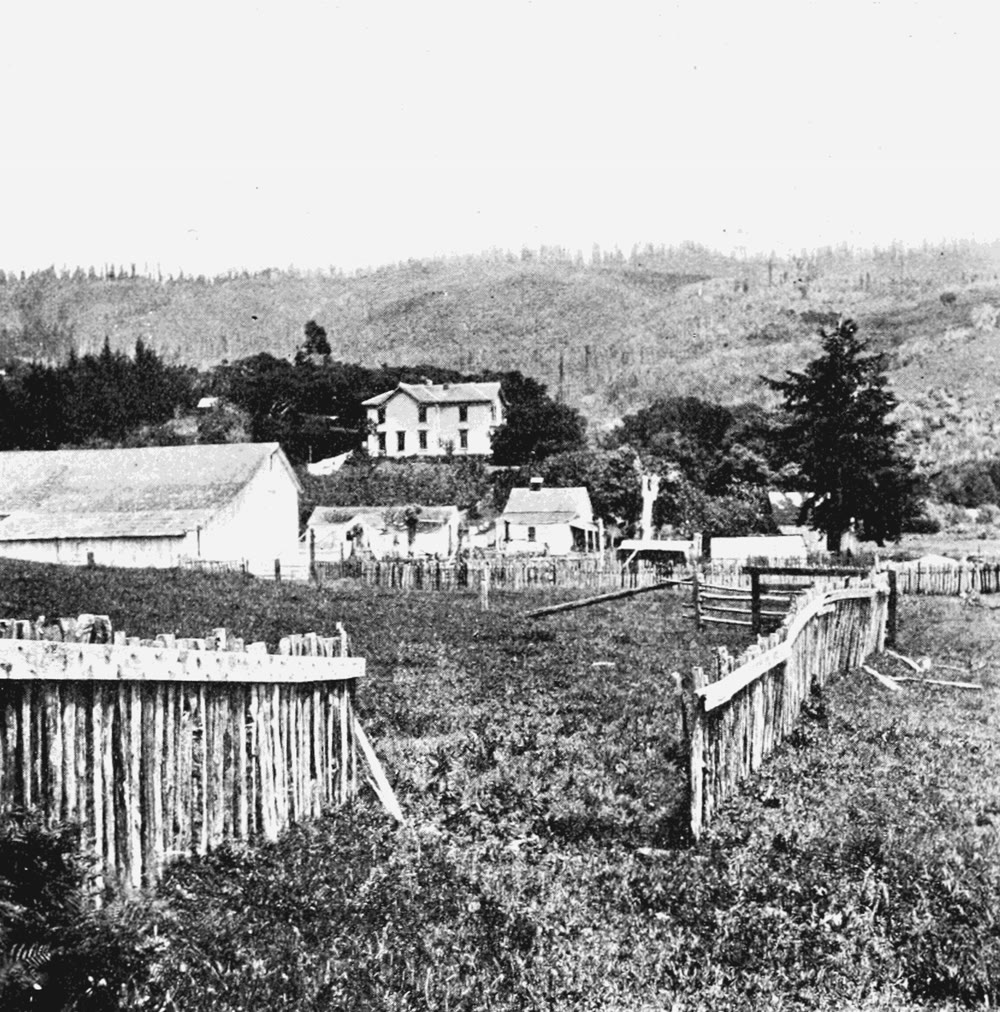
\includegraphics[height=5.6cm]{images/book3/b1-fence-1906.jpg}\hfill
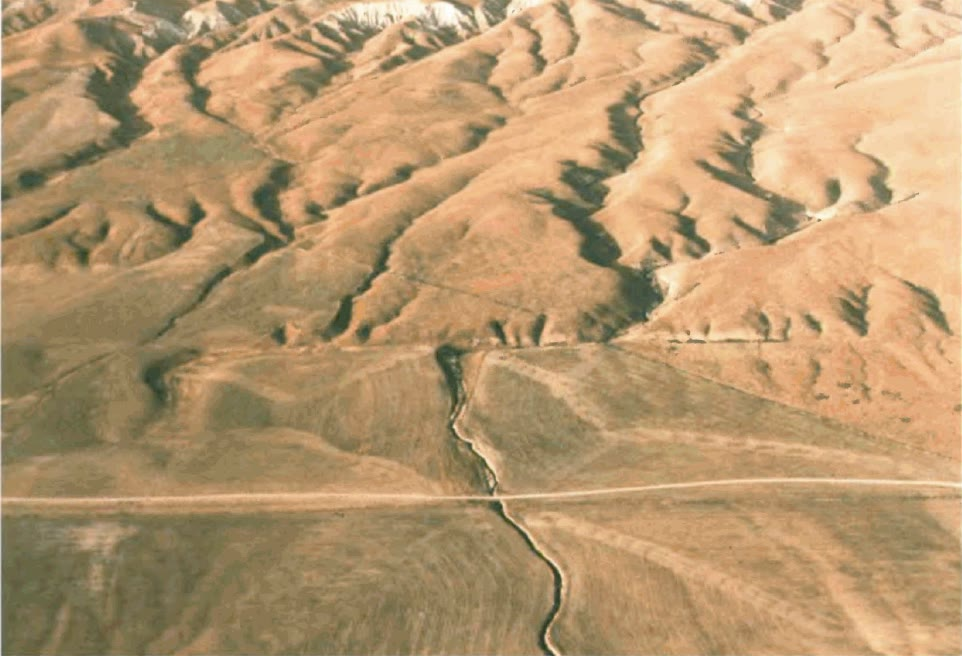
\includegraphics[height=5.6cm]{images/book3/b1-wallace-creek.jpg}
\par\smallskip{\small Izquierda: cercas en tierras de cultivo del condado de Marin, al norte de San Francisco, cruzadas por la rotura de
1906, publicadas el mismo año con el título ``tierra separada por la falla del terremoto''. Fotografía de \emph{Popular Science
Monthly}, vol.~69 (1906), dominio público. Derecha: Wallace Creek, Carrizo Plain, vista desde el aire: el arroyo baja desde las colinas
(arriba), y allí donde cruza la falla de San Andrés, al pie de las colinas, su cauce da un salto lateral de \qty{130}{m}, el
desplazamiento acumulado en miles de años de terremotos. Fotografía: R.~E.~Wallace, Servicio Geológico de los Estados Unidos, dominio
público. Ambas de Wikimedia Commons.}
\label{fig:b1:earthquake-source:offsets}
\end{omfigure}
% ledger: commons:psm-fence, commons:wallace-creek

Cerca de Parkfield, en la misma falla, un terremoto de magnitud alrededor de 6 en 1857 fue seguido de otros cinco, muy parecidos, en el
mismo tramo de unos \qty{30}{km}, a intervalos de casi 22 años hasta 1966; el siguiente se esperaba antes de 1993, y llegó en 2004,
con una \omterm{def:b1:earthquake-source:mw}{magnitud de momento} de 6.0 y sin ninguna señal clara de aviso. La resistencia de una falla, el deslizamiento de cada terremoto
y la carga de sus vecinas varían de un ciclo a otro, y el \omterm{def:b1:earthquake-source:seismic-cycle}{ciclo sísmico} se describe mejor con un intervalo medio de recurrencia y una
dispersión alrededor de él que con un periodo.
% ledger: pp1515:parkfield, bl85:parkfield, usgs:hist-mw, bakun:2005

Algunos segmentos de falla no se bloquean en absoluto. Entre Parkfield y San Juan Bautista, el tramo central de la falla de San Andrés
repta: el deslizamiento constante de la falla absorbe casi todo el movimiento de las placas, y se acumula poca o ninguna deformación a
uno y otro lado, así que este tramo no tiene grandes terremotos; la gran rotura de 1857 empezó en su extremo sur, y la de 1906 se detuvo
en su extremo norte. Una falla que repta sobre parte de su área está bloqueada solo en parte, que es el coeficiente $c$ de la
proposición.
% ledger: pp1515:creep, pp1515:1906

\begin{inthefield}[Leer los terremotos pasados en una trinchera]
Los instrumentos han registrado terremotos durante poco más de un siglo, mucho menos que un ciclo de la mayoría de las fallas. Los
paleosismólogos extienden el registro leyendo el terreno. Se excava una trinchera de unos metros de profundidad a través de una falla
activa donde se han depositado capas de sedimento de forma continua, en un pantano, un lago o un pequeño abanico aluvial. En sus
paredes, cada terremoto aparece como capas cortadas y desplazadas por la falla y cubiertas, sin romper, por otras más recientes; como
una escarpa enterrada por depósitos posteriores; como arena que se licuó y subió por grietas hasta extenderse sobre la superficie de
entonces. La turba o los restos vegetales de las capas justo debajo y justo encima de cada rotura se datan por radiocarbono, y así
acotan la fecha de cada terremoto: un pantano de la falla de San Andrés guarda el registro de doce. A lo largo de las costas, las
capas de arena depositadas por tsunamis y los pantanos que se hundieron de golpe un metro o así, enterrados bajo lodo de marea,
registran los grandes terremotos de subducción. En la falla de San Andrés, la mayor parte del deslizamiento de tiempos históricos llegó
con terremotos de magnitud 6 o más.
\end{inthefield}
% ledger: pp1515:pallett, atwater:1987

\begin{history}[Harry Fielding Reid y el rebote elástico]
Harry Fielding Reid, físico estadounidense, formó parte de la comisión estatal que estudió el terremoto de 1906. Al comparar las
posiciones de puntos topografiados en 1851--1865, en 1874--1892 y después del terremoto, encontró que puntos lejanos a uno y otro lado
de la falla de San Andrés se habían desplazado unos \qty{3.2}{m} uno respecto del otro desde el primer levantamiento, algo más de la
mitad del deslizamiento de unos \qty{6}{m} en la falla: medio siglo antes del terremoto, la deformación que rompió la falla ya estaba
a la mitad de su carga. Solo las fuerzas elásticas podían haber movido el terreno tan de repente, y llamó a ese retorno súbito \omterm{def:b1:earthquake-source:seismic-cycle}{rebote
elástico}. Lo publicó en el segundo volumen del informe de la comisión, en 1910; sigue siendo el modelo principal del \omterm{def:b1:earthquake-source:seismic-cycle}{ciclo sísmico}.
La posición por satélite ha medido después la flexión que él solo podía inferir.
\end{history}
% ledger: reid:1910, pp1515:1906

\section{Momento sísmico y magnitud}\label{sec:b1:earthquake-source:moment}

El tamaño de un terremoto es la cantidad de deslizamiento que produjo, sobre el área de falla que deslizó, ponderada por la rigidez de
las rocas.

\begin{definition}[Momento sísmico]\label{def:b1:earthquake-source:moment}
Sea un terremoto que desliza la cantidad media $D$ sobre una rotura de área $A$, en rocas de módulo de cizalla $\mu$ (la letra
designa también un coeficiente de fricción, en \cref{ch:b1:stress-strain-rheology}; el contexto dice cuál). Su \emph{momento sísmico}\index{momento sísmico}
es
\[
  M_0 = \mu A D ,
\]
en newton metros.
\end{definition}
% ledger: usgs:gloss-moment

La unidad es la de un par de fuerzas. Un deslizamiento sobre una falla emite las mismas ondas que dos pares de fuerzas opuestas,
dos pares de fuerzas, aplicados en el foco, y el \omterm{def:b1:earthquake-source:moment}{momento sísmico} es el momento de cada par (esta equivalencia, el doble par, se
demuestra en el volumen del año~3). El momento tiene las dimensiones de una energía, pero no es una energía: la energía irradiada
como ondas es una pequeña fracción de él. Para las rocas de la \omterm{def:b1:layered-earth:layers}{corteza}, $\mu$ se toma como \qty{30}{GPa}.
% ledger: kanamori:1977, sk:mu-locking

El momento se calcula hoy a partir de las ondas de periodo largo registradas en todo el mundo. Para el terremoto de Tohoku, del 11 de
marzo de 2011, la solución preferida del Servicio Geológico de los Estados Unidos da $M_0 = \qty{5.59e22}{N.m}$. La falla deslizó sobre
un área de unos \qty{400}{km} de longitud y \qty{150}{km} de anchura; la definición da entonces el deslizamiento medio
\[
  D = \frac{M_0}{\mu A}
    = \frac{\num{5.59e22}}{\num{3e10}\times\num{4e5}\times\num{1.5e5}}
    \approx \qty{31}{m} ,
\]
y los modelos de la rotura encuentran hasta \qtyrange{50}{60}{m} en su parte más desplazada.
% ledger: usgs:tohoku-mt, usgs:tohoku-summary

La magnitud de la que trata el libro 1 se calculaba a partir de la amplitud de las ondas en un sismograma. Tales magnitudes miden las
ondas de un periodo; una vez que una rotura es mucho más larga que su longitud de onda, de unos pocos a unos cincuenta kilómetros, la
amplitud deja de crecer con su tamaño, y la magnitud se satura. La magnitud de ondas de volumen se satura cerca de 6.5, la magnitud de
ondas superficiales cerca de 8.3. En 2011, el primer aviso de tsunami para Tohoku se basó en una magnitud de este tipo, que se queda
corta para terremotos de magnitud 8 o más, y subestimó las ondas. El momento no se satura, y la magnitud se define hoy a partir de él.
% ledger: kanamori:1977, usgs:magtypes, jma:warning

\begin{definition}[Magnitud de momento]\label{def:b1:earthquake-source:mw}
La \emph{magnitud de momento}\index{magnitud de momento} de un terremoto de \omterm{def:b1:earthquake-source:moment}{momento sísmico} $M_0$, en newton metros, es
\[
  M_w = \tfrac23\left(\log_{10} M_0 - 9.1\right) .
\]
\end{definition}
% ledger: usgs:magtypes

Thomas Hanks y Hiroo Kanamori definieron la escala en 1979, con la constante 9.05 en lugar de 9.1, una diferencia de 0.03 en $M_w$; las
constantes se eligieron para coincidir con las magnitudes antiguas donde estas no se saturan. La magnitud del libro 1 es, para los
grandes terremotos, este número: para Tohoku,
$M_w = \tfrac23(\log_{10}\num{5.59e22} - 9.1) = \tfrac23(22.75 - 9.1) = 9.1$;
los grandes terremotos chileno de 1960 y de Alaska de 1964 tienen \omterm{def:b1:earthquake-source:mw}{magnitudes de momento} de 9.5 y 9.2, tamaños que las magnitudes
antiguas no podían mostrar.
% ledger: hk:1979, kanamori:1977, usgs:hist-mw, usgs:tohoku-mt

\begin{proposition}[Una unidad de magnitud]\label{prop:b1:earthquake-source:moment-steps}
El \omterm{def:b1:earthquake-source:moment}{momento sísmico} es $M_0 = 10^{1.5 M_w + 9.1}$ newton metros. Una unidad de \omterm{def:b1:earthquake-source:mw}{magnitud de momento} lo multiplica por $10^{1.5} \approx 31.6$,
dos unidades por $1000$. Si la energía irradiada es una fracción fija del momento, crece en la misma proporción.
\end{proposition}

\begin{proof}
Al despejar $M_0$ en la definición se obtiene $\log_{10} M_0 = 1.5 M_w + 9.1$,
y para dos terremotos
\[
  \log_{10}\frac{M_0'}{M_0} = 1.5\,(M_w' - M_w) ,
\]
que vale $1.5$ para una unidad y $3$ para dos. Si la energía irradiada es $E_s = k M_0$ con la misma $k$
para ambos, $E_s'/E_s = M_0'/M_0$.
\end{proof}

La aproximación de Kanamori, $E_s \approx M_0/(2\times10^4)$ (admitida), es la hipótesis de la última frase; el factor de unos 32 en
energía por unidad de magnitud, que se encontró en el libro 1, es esta proposición. Como $M_0 = \mu A D$ y el deslizamiento de un
terremoto crece con el tamaño de su rotura, una magnitud grande necesita una falla grande. La rotura de 1906, de unos \qty{430}{km} de
longitud, rompió la \omterm{def:b1:stress-strain-rheology:strength-envelope}{capa sismogénica} hasta unos \qty{15}{km} con un deslizamiento medio de unos metros: con $D = \qty{4}{m}$,
$M_0 = \num{3e10}\times\num{4.3e5}\times\num{1.5e4}
\times 4 = \qty{7.7e20}{N.m}$ y $M_w = 7.9$, la magnitud del catálogo. Una magnitud de 9 necesita una rotura de cientos de kilómetros de
longitud y más de cien de anchura, que solo ofrecen las interfases de poca pendiente de las zonas de subducción.
% ledger: kanamori:1977, pp1515:1906, usgs:hist-mw, usgs:pp1515-thatcher

\section{Mecanismos focales}\label{sec:b1:earthquake-source:focal}

La onda P es la primera en llegar a un sismómetro. Su \omterm{def:b1:earthquake-source:focal-mechanism}{primer movimiento}, el primer desplazamiento del registro vertical, es hacia
arriba donde la onda llega como un empuje, con el terreno comprimido y alejado de la fuente, y hacia abajo donde llega como un tirón.
Alrededor de un terremoto, los empujes y los tirones se disponen en un patrón que da la orientación de la falla y la dirección del
deslizamiento.

\begin{proposition}[El signo del primer movimiento]\label{prop:b1:earthquake-source:first-motion}
Sea una falla de normal hacia arriba $\mathbf n$ que desliza según el vector unitario $\mathbf d$ (el deslizamiento del \omterm{def:b1:faults-folds-fabrics:fault-elements}{bloque
superior} respecto del \omterm{def:b1:faults-folds-fabrics:fault-elements}{bloque inferior}). La onda P que sale del foco en la dirección unitaria $\mathbf x$ llega como un empuje si
$(\mathbf n\cdot\mathbf x)(\mathbf d\cdot\mathbf x) > 0$ y como un tirón si
$(\mathbf n\cdot\mathbf x)(\mathbf d\cdot\mathbf x) < 0$. Los empujes y los
tirones llenan así cuatro cuadrantes, separados por el plano de la falla
($\mathbf n\cdot\mathbf x = 0$) y por el plano perpendicular al deslizamiento
($\mathbf d\cdot\mathbf x = 0$).
\end{proposition}

\begin{proof}
Una dirección con $\mathbf n\cdot\mathbf x > 0$ apunta hacia el \omterm{def:b1:faults-folds-fabrics:fault-elements}{bloque superior}, que se mueve $\mathbf d$ respecto del \omterm{def:b1:faults-folds-fabrics:fault-elements}{bloque inferior}:
la roca delante de ella, donde $\mathbf d\cdot\mathbf x > 0$, está comprimida, y la roca detrás, donde $\mathbf d\cdot\mathbf x < 0$, es
estirada. Una dirección con $\mathbf n\cdot\mathbf x < 0$ apunta hacia el \omterm{def:b1:faults-folds-fabrics:fault-elements}{bloque inferior}, que se mueve según
$-\mathbf d$ respecto del \omterm{def:b1:faults-folds-fabrics:fault-elements}{bloque superior}, así que los signos se invierten. En cada caso el \omterm{def:b1:earthquake-source:focal-mechanism}{primer movimiento} tiene el signo de $(\mathbf n\cdot\mathbf x)(\mathbf
d\cdot\mathbf x)$.
\end{proof}

El argumento da solo el signo. La amplitud del \omterm{def:b1:earthquake-source:focal-mechanism}{primer movimiento}, que es proporcional a $2(\mathbf n\cdot\mathbf x)(\mathbf d\cdot\mathbf x)$
y por tanto mayor a \ang{45} de ambos planos y nula sobre ellos, se admite aquí (volumen del año~3).

\begin{omfigure}
\begin{tikzpicture}[>={Stealth[length=5pt]}, font=\small, scale=0.95]
% map view around a vertical dextral fault striking north, the focus at the origin, rays leaving
% horizontally: pushes where (n.x)(d.x) > 0, i.e. in the NW and SE quadrants (beachballs.py,
% first_motion(0, 90, 180, x)). Stations at 20 azimuths on a circle of radius 2.3.
\fill[omThm!22] (0,0) -- (0,2.8) arc[start angle=90, end angle=180, radius=2.8] -- cycle;
\fill[omThm!22] (0,0) -- (0,-2.8) arc[start angle=270, end angle=360, radius=2.8] -- cycle;
\draw[black!40, line width=0.4pt] (0,0) circle[radius=2.8];
\draw[fault, line width=1.3pt] (0,-3.1) -- (0,3.1) node[above, font=\scriptsize] {falla (plano nodal)};
\draw[black, dashed, line width=0.7pt] (-3.1,0) -- (3.1,0) node[right, font=\scriptsize, align=left] {plano\\ auxiliar};
% slip: the west block moves north, the east block south
\draw[->, line width=1pt] (-0.3,-0.8) -- (-0.3,0.8);
\draw[->, line width=1pt] (0.3,0.8) -- (0.3,-0.8);
% stations
\foreach \a in {9,27,...,351} {
  \pgfmathsetmacro{\fm}{-sin(\a)*cos(\a)}  % (n.x)(d.x) with n = east, d = south, x = (sin a, cos a)
  \pgfmathparse{\fm>0 ? 1 : 0}
  \ifnum\pgfmathresult=1
    \fill[black] ({2.3*sin(\a)},{2.3*cos(\a)}) circle[radius=0.11];
  \else
    \draw[black, fill=white, line width=0.6pt] ({2.3*sin(\a)},{2.3*cos(\a)}) circle[radius=0.11];
  \fi
}
% P and T axes
\draw[<-, omProp, line width=1.1pt] ({0.7*sin(45)},{0.7*cos(45)}) -- ({1.6*sin(45)},{1.6*cos(45)}) node[above right, font=\scriptsize, inner sep=1pt] {P};
\draw[<-, omProp, line width=1.1pt] ({0.7*sin(225)},{0.7*cos(225)}) -- ({1.6*sin(225)},{1.6*cos(225)});
\draw[->, omProp, line width=1.1pt] ({0.7*sin(315)},{0.7*cos(315)}) -- ({1.6*sin(315)},{1.6*cos(315)}) node[above left, font=\scriptsize, inner sep=1pt] {T};
\draw[->, omProp, line width=1.1pt] ({0.7*sin(135)},{0.7*cos(135)}) -- ({1.6*sin(135)},{1.6*cos(135)});
\fill (0,0) circle[radius=0.06];
% legend
\begin{scope}[xshift=4.6cm, yshift=2.4cm]
  \fill[black] (0,0) circle[radius=0.11]; \node[anchor=west, font=\scriptsize] at (0.2,0) {compresión: primer movimiento hacia arriba};
  \draw[black, fill=white, line width=0.6pt] (0,-0.5) circle[radius=0.11]; \node[anchor=west, font=\scriptsize] at (0.2,-0.5) {dilatación: primer movimiento hacia abajo};
  \fill[omThm!22] (-0.12,-1.12) rectangle (0.12,-0.88); \node[anchor=west, font=\scriptsize] at (0.2,-1.0) {cuadrante de compresión};
  \draw[->] (-0.1,-1.6) -- (-0.1,-1.25); \node[anchor=west, font=\scriptsize] at (0.2,-1.42) {N};
\end{scope}
\end{tikzpicture}
\par\smallskip{\small Primeros movimientos alrededor de una falla \omterm{def:b1:faults-folds-fabrics:fault-types}{dextral} vertical de \omterm{def:b1:geological-maps:attitude}{rumbo} norte, vista desde arriba, para ondas que
salen del foco horizontalmente hacia estaciones situadas todo alrededor. Flechas negras: el deslizamiento de los dos bloques. Los
empujes llenan los cuadrantes noroeste y sudeste, los tirones los otros dos; la falla y el \omterm{def:b1:earthquake-source:focal-mechanism}{plano auxiliar} los separan. El \omterm{def:b1:earthquake-source:focal-mechanism}{eje P} (flechas
que entran) biseca los cuadrantes de tirón, el \omterm{def:b1:earthquake-source:focal-mechanism}{eje T} (flechas que salen) los cuadrantes de empuje. Un deslizamiento \omterm{def:b1:faults-folds-fabrics:fault-types}{sinistral} sobre el
plano discontinuo, con el bloque al sur moviéndose hacia el este, daría exactamente el mismo patrón
(\cref{prop:b1:earthquake-source:auxiliary}).}
\label{fig:b1:earthquake-source:quadrants}
\end{omfigure}

El producto $(\mathbf n\cdot\mathbf x)(\mathbf d\cdot\mathbf x)$ no cambia cuando se intercambian $\mathbf n$ y $\mathbf d$. Esta simetría
es el hecho central de los \omterm{def:b1:earthquake-source:focal-mechanism}{mecanismos focales}.

\begin{definition}[Mecanismo focal, plano nodal, plano auxiliar, eje P, eje T]\label{def:b1:earthquake-source:focal-mechanism}
El \emph{primer movimiento}\index{primer movimiento} de una onda P en un sismómetro es la dirección, hacia arriba o hacia abajo, del
primer desplazamiento del terreno en el registro vertical. El \emph{mecanismo focal}\index{mecanismo focal} de un terremoto es la
orientación del plano de la falla y la dirección del deslizamiento sobre él, tal como se deducen de sus ondas sísmicas. Los dos planos
perpendiculares que pasan por el foco y separan los empujes de los tirones son sus \emph{planos nodales}\index{plano nodal}; uno es el
plano de la falla, y el otro, perpendicular al deslizamiento, es el \emph{plano auxiliar}\index{plano auxiliar}. El \emph{eje
P}\index{eje P} y el \emph{eje T}\index{eje T} son las direcciones a \ang{45} de ambos planos nodales, en el centro de los cuadrantes
de tirón y de los cuadrantes de empuje, respectivamente:
\[
  \mathbf P = \frac{\mathbf n - \mathbf d}{\sqrt2}, \qquad
  \mathbf T = \frac{\mathbf n + \mathbf d}{\sqrt2} .
\]
\end{definition}
% ledger: yvo:beachball, usgs:gloss-moment

\begin{proposition}[Los dos planos nodales]\label{prop:b1:earthquake-source:auxiliary}
Un deslizamiento $\mathbf d$ sobre el plano de normal $\mathbf n$ y un deslizamiento $\mathbf n$ sobre el plano de normal $\mathbf d$
dan los mismos primeros movimientos en cada dirección. Los primeros movimientos determinan, por tanto, los dos \omterm{def:b1:earthquake-source:focal-mechanism}{planos nodales}, los \omterm{def:b1:earthquake-source:focal-mechanism}{ejes P} y T
y el sentido del deslizamiento sobre cada plano, pero no dicen cuál \omterm{def:b1:earthquake-source:focal-mechanism}{plano nodal} es la falla.
\end{proposition}

\begin{proof}
El signo de $(\mathbf n\cdot\mathbf x)(\mathbf d\cdot\mathbf x)$ no cambia por el intercambio de $\mathbf n$ y $\mathbf d$; los planos
$\mathbf n\cdot\mathbf x = 0$ y $\mathbf d\cdot\mathbf x = 0$ se intercambian,
y $\mathbf n \pm \mathbf d$ no cambian. Un par $(\mathbf n, \mathbf d)$ y
el par $(-\mathbf n, -\mathbf d)$, que describe el mismo deslizamiento visto desde el otro bloque, dan también el mismo producto. Nada en los
primeros movimientos distingue las dos descripciones.
\end{proof}

Para decidir qué \omterm{def:b1:earthquake-source:focal-mechanism}{plano nodal} deslizó, los sismólogos usan otras pruebas: el plano a lo largo del cual se alinean las réplicas, la falla vista
en la superficie, el límite de placas en el que yace el terremoto. Para el gran terremoto de Sumatra--Andamán de 2004, los dos \omterm{def:b1:earthquake-source:focal-mechanism}{planos
nodales} buzan \ang{8} hacia el nordeste y \ang{83} hacia el suroeste. Los terremotos anteriores de la región y los modelos de placas sitúan
la losa que se hunde a lo largo de un plano que buza suavemente hacia el nordeste, y se toma el plano somero como la falla: el terremoto
rompió la interfase de placas de la zona de subducción, y sus réplicas se extendieron sobre más de \qty{1300}{km}.
% ledger: usgs:sumatra-mt, usgs:sumatra-summary

Como el \omterm{def:b1:earthquake-source:focal-mechanism}{eje P} yace en el centro de los tirones y el \omterm{def:b1:earthquake-source:focal-mechanism}{eje T} en el centro de los empujes, a menudo se leen como las direcciones del esfuerzo
de compresión mayor y menor, $\sigma_1$ y $\sigma_3$. Son solo aproximaciones de ellos. Una falla nueva se forma a $\ang{45} - \phi/2$ de
$\sigma_1$, no a \ang{45} (\cref{ch:b1:stress-strain-rheology}), y una falla antigua puede deslizar a un ángulo todavía distinto, de modo que los ejes de un
terremoto pueden quedar a decenas de grados de los \omterm{def:b1:stress-strain-rheology:principal}{esfuerzos principales}; los esfuerzos de una región se hallan a partir de los mecanismos de
muchos terremotos juntos.

Un \omterm{def:b1:earthquake-source:focal-mechanism}{mecanismo focal} vive sobre una esfera alrededor del foco. Se dibuja en la mitad inferior de esa esfera, que cruza todo rayo hacia una
estación lejana, proyectada sobre un disco: un rayo de vector unitario $\mathbf x = (E, N, U)$, con $U \le 0$, se dibuja en
\[
  (X, Y) = \frac{(E, N)}{\sqrt{1 - U}} ,
\]
la vertical en el centro y la horizontal sobre el círculo unitario. Esta proyección conserva las áreas (admitido; las proyecciones de la
esfera se estudian en el volumen del año~3), de modo que cada cuadrante ocupa su parte verdadera del disco. Los cuadrantes de empuje se
sombrean; el dibujo se llama pelota de playa.
% ledger: yvo:beachball

\begin{omfigure}
\begin{tikzpicture}[font=\small]
% lower-hemisphere equal-area beach balls, compressional quadrants shaded (figdata/bachelor-1/beachballs.py)
\foreach \n/\c/\t/\x in {normal/2/{(a) falla normal\\ $090/60$, cabeceo \ang{-90}}/0,
                         reverse/1/{(b) falla inversa\\ $090/30$, cabeceo \ang{90}}/3.65,
                         strikeslip/2/{(c) falla de desgarre\\ $090/90$, cabeceo \ang{180}}/7.3,
                         tohoku/2/{(d) Tohoku, 2011\\ $282/8$, cabeceo \ang{78}}/10.95} {
  \begin{axis}[at={(\x cm,0)}, anchor=center, width=2.9cm, height=2.9cm, scale only axis,
      axis equal image, xmin=-1.04, xmax=1.04, ymin=-1.04, ymax=1.04, hide axis, clip=false]
    \fill[white] (axis cs:0,0) circle[radius=1];
    \addplot[fill=omThm!55, draw=none] table[x=X, y=Y] {figdata/out/bachelor-1-beachballs-\n-c1.dat};
    \ifnum\c=2
      \addplot[fill=omThm!55, draw=none] table[x=X, y=Y] {figdata/out/bachelor-1-beachballs-\n-c2.dat};
    \fi
    \addplot[black, line width=0.6pt] table[x=X, y=Y] {figdata/out/bachelor-1-beachballs-\n-p1.dat};
    \addplot[black, line width=0.6pt] table[x=X, y=Y] {figdata/out/bachelor-1-beachballs-\n-p2.dat};
    \draw[black, line width=0.8pt] (axis cs:0,0) circle[radius=1];
    \draw[black, line width=0.5pt] (axis cs:0,1) -- (axis cs:0,1.12) node[above, font=\scriptsize, inner sep=1pt] {N};
    \addplot[only marks, mark=none, nodes near coords={\textbf{P}}, nodes near coords align=center, every node near coord/.append style={font=\scriptsize, inner sep=0pt}] table[x=X, y=Y] {figdata/out/bachelor-1-beachballs-\n-P.dat};
    \addplot[only marks, mark=none, nodes near coords={\textbf{T}}, nodes near coords align=center, every node near coord/.append style={font=\scriptsize, inner sep=0pt}] table[x=X, y=Y] {figdata/out/bachelor-1-beachballs-\n-T.dat};
    \node[anchor=north, align=center, font=\scriptsize] at (axis cs:0,-1.12) {\t};
  \end{axis}
}
\end{tikzpicture}
\par\smallskip{\small Pelotas de playa: la mitad inferior de la esfera alrededor del foco, en proyección de áreas iguales, con el norte
hacia arriba, los cuadrantes de empuje sombreados, y P y T marcando los ejes (una letra se desplaza hacia dentro cuando su eje queda
cerca del borde). Cada mecanismo viene dado por la \omterm{def:b1:geological-maps:attitude}{actitud} de uno de los \omterm{def:b1:earthquake-source:focal-mechanism}{planos nodales}, \omterm{def:b1:geological-maps:attitude}{dirección de buzamiento} y \omterm{def:b1:geological-maps:attitude}{buzamiento}, y el \omterm{def:b1:faults-folds-fabrics:fault-elements}{cabeceo}
del deslizamiento sobre él. (a) Una \omterm{def:b1:faults-folds-fabrics:fault-types}{falla normal} que buza \ang{60} hacia el este: el cuadrante de tirón llena el centro. (b) Una \omterm{def:b1:faults-folds-fabrics:fault-types}{falla
inversa} que buza \ang{30} hacia el este: el cuadrante de empuje llena el centro. (c) Una \omterm{def:b1:faults-folds-fabrics:fault-types}{falla de desgarre} vertical: cuatro cuadrantes
que se encuentran en el centro. (d) El terremoto de Tohoku de 2011 (tensor de momento del Servicio Geológico de los Estados Unidos): un
\omterm{def:b1:faults-folds-fabrics:fault-types}{cabalgamiento} sobre un plano que buza \ang{8} hacia $282$, bajo Japón, con el \omterm{def:b1:earthquake-source:focal-mechanism}{plano auxiliar} empinado al este.}
\label{fig:b1:earthquake-source:beachballs}
\end{omfigure}
% ledger: usgs:tohoku-mt

Los sismólogos dan un mecanismo por el \omterm{def:b1:geological-maps:attitude}{rumbo}, el \omterm{def:b1:geological-maps:attitude}{buzamiento} y el \omterm{def:b1:faults-folds-fabrics:fault-elements}{cabeceo} de cada \omterm{def:b1:earthquake-source:focal-mechanism}{plano nodal}; el \omterm{def:b1:geological-maps:attitude}{rumbo} es la \omterm{def:b1:geological-maps:attitude}{dirección de buzamiento}
menos \ang{90}, como en \cref{ch:b1:faults-folds-fabrics}. Para Tohoku, los planos son
$192/8/78$ y $24/81/91$ en \omterm{def:b1:geological-maps:attitude}{rumbo}, \omterm{def:b1:geological-maps:attitude}{buzamiento} y \omterm{def:b1:faults-folds-fabrics:fault-elements}{cabeceo}, y los \omterm{def:b1:earthquake-source:focal-mechanism}{ejes P} y T tienen tendencia
$113$ y $296$ e \omterm{def:b1:field-lab-methods-1:trend-plunge}{inmersión} \ang{36} y \ang{53}. El \omterm{def:b1:earthquake-source:focal-mechanism}{plano auxiliar} se deduce del plano de la falla: su normal es $\mathbf d$ y su
deslizamiento es $\mathbf n$, de modo que se halla calculando $\mathbf n$ y $\mathbf d$ a partir del \omterm{def:b1:geological-maps:attitude}{rumbo}, el \omterm{def:b1:geological-maps:attitude}{buzamiento} y el \omterm{def:b1:faults-folds-fabrics:fault-elements}{cabeceo},
intercambiándolos, y leyendo de nuevo el \omterm{def:b1:geological-maps:attitude}{rumbo}, el \omterm{def:b1:geological-maps:attitude}{buzamiento} y el \omterm{def:b1:faults-folds-fabrics:fault-elements}{cabeceo}
(ejercicio~\ref{exo:b1:earthquake-source:7}).
% ledger: usgs:tohoku-mt

\begin{method}[Lectura de un diagrama de pelota de playa]\label{met:b1:earthquake-source:beachball}
\begin{enumerate}
  \item Mírese el centro, que es la vertical. Sombreado (un empuje justo hacia abajo): una componente inversa o de \omterm{def:b1:faults-folds-fabrics:fault-types}{cabalgamiento}; blanco:
        una componente normal. Dos diámetros rectos que se cruzan en el centro: un mecanismo de desgarre.
  \item Hállense los dos \omterm{def:b1:earthquake-source:focal-mechanism}{planos nodales}, las curvas que delimitan los cuadrantes. Un plano que pasa por el centro es vertical; un plano
        buza hacia el lado del centro en el que yace su curva, tanto más suavemente cuanto más cerca del borde está la curva.
  \item Hállese el \omterm{def:b1:earthquake-source:focal-mechanism}{eje T} en el centro de los cuadrantes sombreados y el \omterm{def:b1:earthquake-source:focal-mechanism}{eje P} en el centro de los blancos: el terreno se acortó según P y se
        alargó según T.
  \item Para cada \omterm{def:b1:earthquake-source:focal-mechanism}{plano nodal}, léase o calcúlese el \omterm{def:b1:faults-folds-fabrics:fault-elements}{cabeceo}, y nómbrese la falla que sería con
        \cref{def:b1:faults-folds-fabrics:fault-types}. Los dos planos comparten siempre el sentido del deslizamiento de \omterm{def:b1:geological-maps:attitude}{buzamiento}, normal o
        inverso, y tienen sentidos de desgarre opuestos: un mecanismo de desgarre da un plano \omterm{def:b1:faults-folds-fabrics:fault-types}{dextral} y otro \omterm{def:b1:faults-folds-fabrics:fault-types}{sinistral}.
  \item Elíjase el plano de la falla a partir de las réplicas, de la geología o del límite de placas.
\end{enumerate}
\end{method}

\begin{inthelab}[En un observatorio sismológico]
\begin{minipage}[t]{0.6\linewidth}\vspace{0pt}
Pocos minutos después de un gran terremoto, sus ondas han sido registradas por cientos de estaciones, y los datos llegan a los analistas de
los observatorios casi en tiempo real. Las primeras llegadas de la onda P, que llegan más tarde cuanto más lejos está la estación, se
señalan en los registros para localizar el foco. Después, las ondas largas y lentas registradas en las decenas de minutos siguientes se
comparan con ondas calculadas para fuentes de prueba; la fuente cuyas ondas mejor se ajustan da el tensor de momento, que contiene a la vez
el \omterm{def:b1:earthquake-source:moment}{momento sísmico}, la \omterm{def:b1:earthquake-source:mw}{magnitud de momento} y los dos \omterm{def:b1:earthquake-source:focal-mechanism}{planos nodales}. Para los terremotos pequeños, demasiado débiles para esto, los
analistas leen los primeros movimientos en los registros más cercanos y ajustan a ellos los \omterm{def:b1:earthquake-source:focal-mechanism}{planos nodales}, del modo descrito en esta
sección. Cada solución se publica con sus incertidumbres, y se revisa a medida que llegan más datos.
\end{minipage}\hfill
\begin{minipage}[t]{0.36\linewidth}\vspace{0pt}
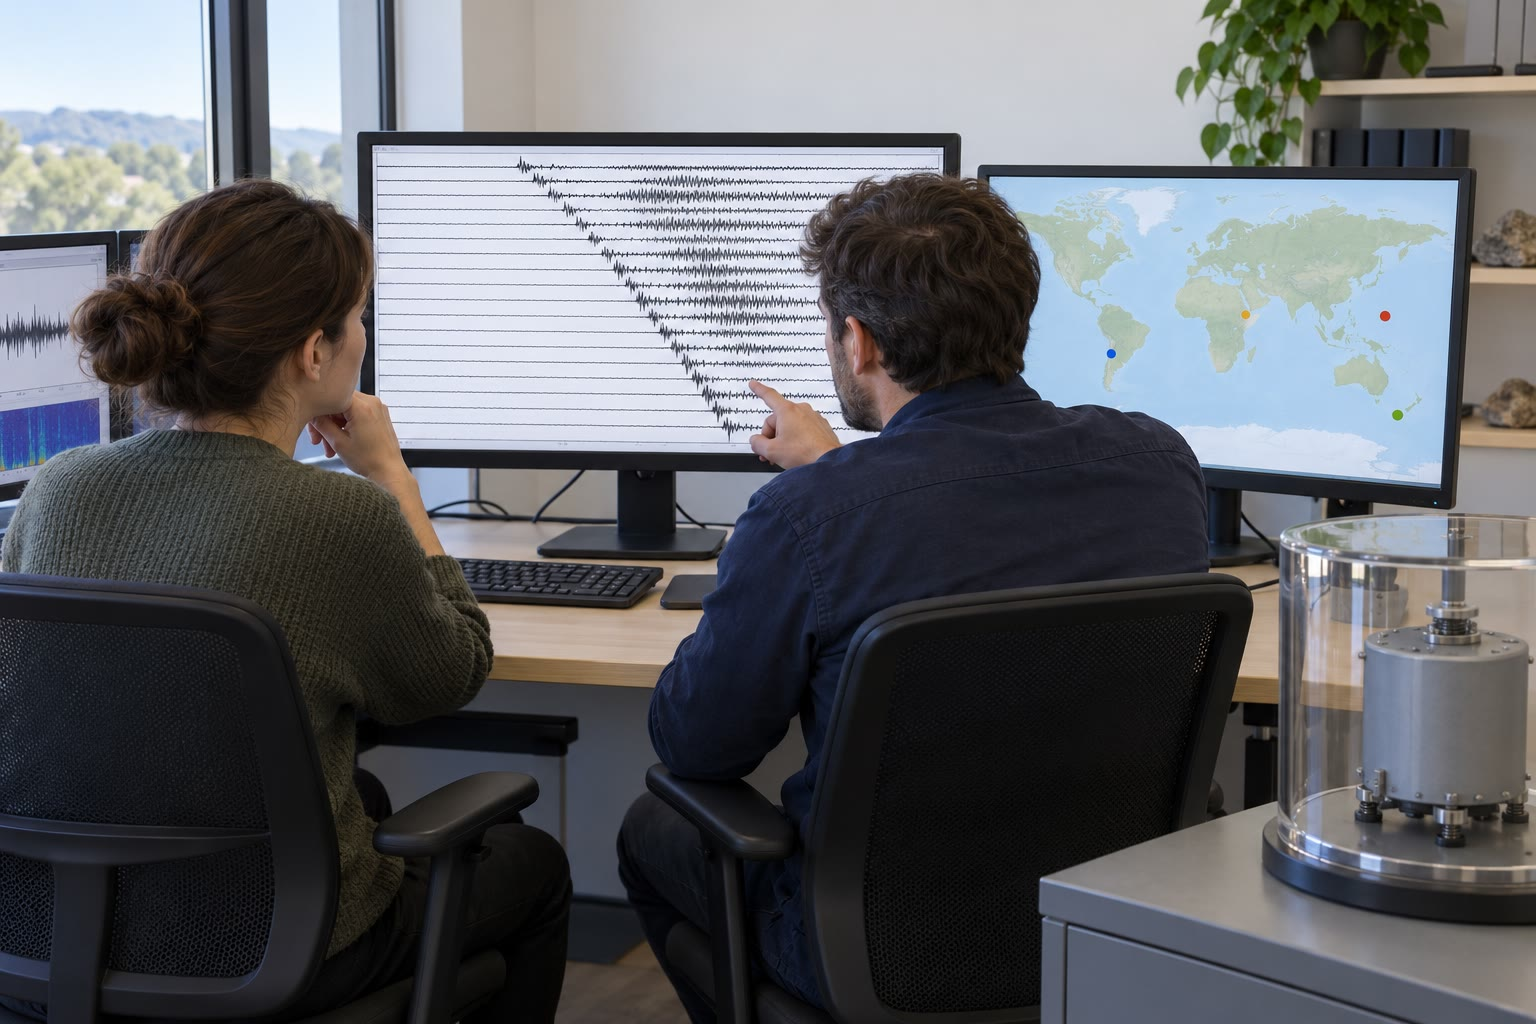
\includegraphics[width=\linewidth]{images/book3/ai/b1-seismic-analysis.jpg}

{\scriptsize Sismólogos leyendo una sección de registros, las trazas de un mismo terremoto en estaciones ordenadas por distancia
(ilustración IA).}
\end{minipage}
\end{inthelab}
% ledger: yvo:beachball

\section{Medir la carga: geodesia}\label{sec:b1:earthquake-source:geodesy}

Entre terremotos, una falla bloqueada es invisible para los sismómetros, pero el terreno a su alrededor se mueve. Las estaciones
permanentes de posicionamiento por satélite miden ese movimiento, y la manera en que cambian sus velocidades a través de una falla indica
hasta qué profundidad está bloqueada.

\begin{definition}[Profundidad de bloqueo]\label{def:b1:earthquake-source:locking-depth}
La \emph{profundidad de bloqueo}\index{profundidad de bloqueo} de una falla es la profundidad hasta la que está bloqueada entre
terremotos, deslizando la falla por debajo de ella de manera constante a la velocidad a largo plazo; es la profundidad de la parte de la
falla que desliza en el siguiente terremoto.
\end{definition}
% ledger: usgs:pp1515-thatcher

\begin{proposition}[Velocidad intersísmica a lo largo de una falla de desgarre]\label{prop:b1:earthquake-source:interseismic}
Sea una \omterm{def:b1:faults-folds-fabrics:fault-types}{falla de desgarre} vertical en un semiespacio elástico, bloqueada desde la superficie hasta la profundidad $D$, y que desliza a la
velocidad $V$ por debajo de ella. La velocidad de la superficie paralela a la falla, a la distancia $x$ de ella, es
\[
  v(x) = \frac{V}{\pi}\arctan\frac{x}{D} .
\]
Si la falla desliza después $s$ desde la superficie hasta la profundidad $D$ en un terremoto, la superficie se mueve $u(x) = (s/\pi)\arctan(D/x)$
para $x > 0$, y $-u(-x)$ para $x < 0$.
\end{proposition}
\admitted

Este modelo, debido a Savage y Burford, es la forma más simple del \omterm{def:b1:earthquake-source:seismic-cycle}{rebote elástico}, y la curva de la cerca de la primera figura. Sus
propiedades se siguen de la fórmula.

\begin{proposition}[Lectura del perfil intersísmico]\label{prop:b1:earthquake-source:profile}
En el modelo de \cref{prop:b1:earthquake-source:interseismic}:
\begin{enumerate}[label=(\alph*)]
  \item lejos de la falla la velocidad tiende a $\pm V/2$, moviéndose las dos placas a $V$ una respecto de la otra;
  \item la mitad del cambio de velocidad a través de la falla ocurre a una distancia $D$ de ella: $v(\pm D) = \pm V/4$;
  \item la velocidad de \omterm{def:b1:stress-strain-rheology:strain}{deformación de cizalla} de la superficie, $\mathrm dv/\mathrm dx$, es mayor sobre la falla, donde vale $V/(\pi D)$;
  \item si la falla, tras cargar durante el tiempo $t$, desliza $s = Vt$ en un terremoto, el terreno acaba desplazado $\pm s/2$ en todas
        partes a uno y otro lado: el ciclo no deja flexión permanente, solo el desplazamiento $s$ sobre la falla.
\end{enumerate}
\end{proposition}

\begin{proof}
(a) $\arctan(x/D) \to \pm\pi/2$ cuando $x \to \pm\infty$. (b) $\arctan 1 = \pi/4$,
así que $v(D) = V/4$, y $v$ es impar. (c) $\mathrm dv/\mathrm dx = (V/\pi D)/(1 +
x^2/D^2)$, mayor en $x = 0$. (d) Para $x > 0$, la carga ha desplazado el
terreno $t\,v(x) = (s/\pi)\arctan(x/D)$ y el terremoto $(s/\pi)\arctan(D/x)$;
como $\arctan y + \arctan(1/y) = \pi/2$ para $y > 0$, la suma es $s/2$. Lo mismo
vale con los signos invertidos para $x < 0$.
\end{proof}

La propiedad (b) da la \omterm{def:b1:earthquake-source:locking-depth}{profundidad de bloqueo} a partir de un perfil de estaciones: es la distancia a la falla a la que la velocidad ha
cambiado en un cuarto de $V$ respecto de su valor sobre la falla. Un bloqueo somero concentra la deformación cerca de la falla (la figura
de abajo), y uno profundo la reparte en una banda ancha. A lo largo del sistema de San Andrés, las \omterm{def:b1:earthquake-source:locking-depth}{profundidades de bloqueo} halladas por
geodesia van de casi 0, en los tramos que reptan, a \qty{26}{km}, y concuerdan con las profundidades de los terremotos: la parte bloqueada es
la \omterm{def:b1:stress-strain-rheology:strength-envelope}{capa sismogénica} de \cref{ch:b1:stress-strain-rheology}. Para una velocidad de deslizamiento de \qty{34}{mm.yr^{-1}} y una \omterm{def:b1:earthquake-source:locking-depth}{profundidad de
bloqueo} de \qty{15}{km}, la velocidad de \omterm{def:b1:stress-strain-rheology:strain}{deformación de cizalla} sobre la falla es $\num{0.034}/(\pi\times\num{15000}) = \num{7.2e-7}$ por año,
que dobla una línea que cruza la falla en menos de un milímetro por kilómetro al año, pero que acumula, en dos siglos, los varios metros de
deslizamiento de un gran terremoto.
% ledger: sk:mu-locking, usgs:pp1515-wallace, usgs:pp1515-thatcher

\begin{omfigure}
\begin{tikzpicture}[font=\small]
\begin{axis}[omrecord, width=11cm, height=5.6cm, xmin=-100, xmax=100, ymin=-19, ymax=19,
  xlabel={distancia a la falla $x$ (km)}, ylabel={velocidad $v$ (\unit{mm.yr^{-1}})},
    legend style={font=\scriptsize, at={(0.02,0.96)}, anchor=north west}, legend cell align=left]
  \addplot[omDef, line width=0.9pt, dashed] table[x=x, y=v5] {figdata/out/bachelor-1-interseismic-profiles.dat};
  \addplot[omThm, line width=1.1pt] table[x=x, y=v15] {figdata/out/bachelor-1-interseismic-profiles.dat};
  \addplot[omProp, line width=0.9pt, dotted] table[x=x, y=v25] {figdata/out/bachelor-1-interseismic-profiles.dat};
  \legend{$D = \qty{5}{km}$, $D = \qty{15}{km}$, $D = \qty{25}{km}$}
  \draw[black!50, dashed] (axis cs:-100,17) -- (axis cs:100,17);
  \draw[black!50, dashed] (axis cs:-100,-17) -- (axis cs:100,-17);
  \node[anchor=north west, font=\scriptsize] at (axis cs:-30,17) {$+V/2$};
  \node[anchor=south west, font=\scriptsize] at (axis cs:30,-17) {$-V/2$};
  \draw[black!60] (axis cs:0,-19) -- (axis cs:0,19);
  \node[anchor=east, font=\scriptsize] at (axis cs:-1,5) {falla};
\end{axis}
\end{tikzpicture}
\par\smallskip{\small Velocidad del terreno paralela a una \omterm{def:b1:faults-folds-fabrics:fault-types}{falla de desgarre} bloqueada, respecto de la traza de la falla, para una velocidad
de deslizamiento $V = \qty{34}{mm.yr^{-1}}$, la de la falla de San Andrés en Wallace Creek, y tres \omterm{def:b1:earthquake-source:locking-depth}{profundidades de bloqueo}
(\cref{prop:b1:earthquake-source:interseismic}). Cuanto más somero es el bloqueo, más estrecha es la banda en la que cambia la velocidad.}
\label{fig:b1:earthquake-source:interseismic}
\end{omfigure}
% ledger: usgs:pp1515-wallace

La posición por satélite mide el terreno en unas pocas estaciones. Los satélites de radar lo miden en todas partes: dos imágenes de radar de
la misma zona tomadas desde la misma órbita en momentos distintos se comparan onda a onda, y la diferencia de fase cartografía el cambio de
la distancia entre el terreno y el satélite, punto a punto, cada cien metros, sin necesidad de una red de estaciones instalada de antemano.
El primer mapa de este tipo, de un gran terremoto californiano de 1992, mostró su desplazamiento cosísmico en una sola imagen y concordó con
el deslizamiento medido sobre el terreno y con topografía; la técnica, la interferometría de radar, pertenece al volumen del año~3.
% ledger: massonnet:1993

\section{Con qué frecuencia: la ley de Gutenberg--Richter}\label{sec:b1:earthquake-source:gr}

Los terremotos pequeños son mucho más comunes que los grandes, y de una manera notablemente regular.

\begin{proposition}[Ley de Gutenberg--Richter]\label{prop:b1:earthquake-source:gutenberg-richter}
En una región y un periodo\index{ley de Gutenberg--Richter}, el número $N$ de terremotos de magnitud al menos
$M$ sigue
\[
  \log_{10} N = a - bM ,
\]
para todo $M$ por encima de la \omterm{def:b1:earthquake-source:b-value}{magnitud de completitud} del catálogo, con constantes $a$ y $b$ que dependen de la región; $b$ está cerca de 1 en
la mayoría de las regiones activas.
\end{proposition}
\admitted
% ledger: fd:1993, gr:1944

La ley es un resultado de la observación, publicado por Beno Gutenberg y Charles Richter para California en 1944 y encontrado después en
todas partes; ninguna teoría la deduce todavía, ni deduce el valor de $b$.
% ledger: gr:1944

\begin{definition}[Valor b, magnitud de completitud]\label{def:b1:earthquake-source:b-value}
La constante $b$ de la \omterm{prop:b1:earthquake-source:gutenberg-richter}{ley de Gutenberg--Richter} de una región es su
\emph{valor b}\index{valor b}. La \emph{magnitud de
completitud}\index{magnitud de completitud} de un catálogo es la menor
magnitud por encima de la cual registra todos los terremotos de la región y el periodo.
\end{definition}

Un \omterm{def:b1:earthquake-source:b-value}{valor b} de 1 significa diez veces menos terremotos por cada unidad de magnitud. Por debajo de la \omterm{def:b1:earthquake-source:b-value}{magnitud de completitud}, los recuentos
quedan por debajo de la recta, porque los terremotos pequeños son registrados por muy pocas estaciones para localizarlos: la ley parece
doblarse, y $b$ debe medirse por encima de ella. Para toda la Tierra, dividida en terremotos someros, intermedios y profundos, los valores
medidos están entre 0.72 y 1.34, pero difieren en un \qty{30}{\percent} o más de un catálogo, intervalo de magnitudes o método a otro: un
valor alejado de 1 es, ante todo, una razón para revisar el catálogo.
% ledger: fd:1993

\begin{omfigure}
\begin{tikzpicture}[font=\small]
\begin{axis}[omrecord, width=6.4cm, height=5.8cm, ymode=log, xmin=5.8, xmax=9.3, ymin=0.01, ymax=300,
  xlabel={magnitud $M$}, ylabel={sucesos de magnitud $\ge M$ por año},
  log basis y=10, title={(a) frecuencia y magnitud}, title style={font=\small}]
  \addplot[omProp, line width=0.9pt, domain=5.8:9.3] table[x=M, y=rate] {figdata/out/bachelor-1-gutenberg_richter-fit.dat};
  \addplot[only marks, mark=*, mark size=1.3pt, omDef] table[x=M, y=rate] {figdata/out/bachelor-1-gutenberg_richter-counts.dat};
  \draw[black!50, dashed] (axis cs:7.5,0.01) -- (axis cs:7.5,300);
  \node[anchor=south west, font=\scriptsize, omProp] at (axis cs:8.45,0.5) {$b = 1.01$};
  \node[anchor=north west, font=\scriptsize, align=left] at (axis cs:7.55,200) {ajuste entre\\ $6.0 \le M \le 7.5$};
\end{axis}
\begin{axis}[omrecord, at={(7.6cm,0)}, width=6.4cm, height=5.8cm, xmin=5.8, xmax=9.3, ymin=0, ymax=1.05,
    xlabel={magnitud $M$}, ylabel={fracción del momento de los sucesos $\ge M$},
    title={(b) adónde va el momento}, title style={font=\small}]
  \addplot[const plot, omDef, line width=0.9pt] table[x=M, y=share] {figdata/out/bachelor-1-gutenberg_richter-moment.dat};
\end{axis}
\end{tikzpicture}
\par\smallskip{\small Los \num{7031} terremotos de magnitud 6 o más en el mundo, de 1976 a 2025 (catálogo del Servicio Geológico de los
Estados Unidos). (a) El número anual de terremotos de magnitud al menos $M$; la recta es el ajuste por mínimos cuadrados de $\log_{10} N$
frente a $M$ entre 6.0 y 7.5, donde cada recuento supera 200: $\log_{10} N = 8.20 - 1.01\,M$ por año. Por encima de la magnitud 8, los pocos
sucesos quedan por debajo de la recta. (b) La fracción del \omterm{def:b1:earthquake-source:moment}{momento sísmico} total liberado por los terremotos de magnitud al menos $M$, cada
momento calculado como $10^{1.5M + 9.1}$\,\unit{N.m}: los 40 terremotos de magnitud 8 o más liberaron el \qty{63}{\percent} de él.}
\label{fig:b1:earthquake-source:gutenberg-richter}
\end{omfigure}
% ledger: data:usgs-comcat (fit and shares computed in figdata/bachelor-1/gutenberg_richter.py)

Para el catálogo mundial de la figura, la ley con $a = 8.20$ y $b = 1.01$ predice 14 terremotos de magnitud 7 o más al año, como se observa,
y 1.35 de magnitud 8 o más, mientras que se registraron 40 en cincuenta años, 0.8 al año. Si los terremotos más grandes son realmente menos
de los que indica la recta, como sugeriría el tamaño finito de las fallas, o solo son lo bastante raros para faltar en cincuenta años, no
queda resuelto con tan pocos sucesos. Alrededor de uno de cada nueve valores de magnitud de este catálogo es una magnitud de ondas
superficiales o de ondas de volumen, que se saturan; los mayores sucesos tienen todos \omterm{def:b1:earthquake-source:mw}{magnitudes de momento}.
% ledger: data:usgs-comcat

Los muchos terremotos pequeños hacen poco del trabajo. Su número crece diez veces por cada unidad de magnitud menos, pero sus momentos se
reducen 31.6 veces.

\begin{proposition}[Los terremotos más grandes liberan la mayor parte del momento]\label{prop:b1:earthquake-source:largest}
Sean los terremotos que siguen la \omterm{prop:b1:earthquake-source:gutenberg-richter}{ley de Gutenberg--Richter} con $b < 1.5$, hasta una magnitud máxima $M_{\max}$, y agrupados en intervalos
de una unidad de magnitud de ancho, terminando el intervalo superior en $M_{\max}$. Entonces los terremotos del intervalo superior liberan más
de la fracción $1 - 10^{-(1.5 - b)}$ del momento total, por pequeña que sea la menor magnitud contada: más del \qty{68}{\percent} para $b = 1$.
\end{proposition}

\begin{proof}
Numérense los intervalos $k = 0, 1, \dots, K$ desde el menor, yendo el intervalo $k$ de $M_k$ a $M_k + 1$, con $M_{k+1} = M_k + 1$. Por la ley, el número
de terremotos en el intervalo $k$ es $10^{a - bM_k} - 10^{a - b(M_k+1)} =
10^{a - bM_k}(1 - 10^{-b})$; por \cref{prop:b1:earthquake-source:moment-steps}
el momento de cada uno está entre $10^{1.5M_k + 9.1}$ y $10^{1.5}$ veces eso,
y como cada intervalo es el anterior desplazado una unidad, el momento del
intervalo $k$ es $C q^k$ para una constante $C$, y el cociente
$q = 10^{-b}\times10^{1.5} = 10^{1.5 - b} > 1$. El total es la suma geométrica
\[
  S = C(1 + q + \dots + q^K) = C\,\frac{q^{K+1} - 1}{q - 1} ,
\]
y la fracción del intervalo superior es
\[
  \frac{C q^K}{S} = \frac{q^K (q - 1)}{q^{K+1} - 1}
  > \frac{q^K (q - 1)}{q^{K+1}} = 1 - \frac1q = 1 - 10^{-(1.5 - b)} .
\]
Para $b = 1$, $1 - 10^{-0.5} = 0.684$.
\end{proof}

En el catálogo mundial la fracción es de este orden: la unidad superior de magnitud, de 8.1 a 9.1, liberó más de la mitad del momento de
cincuenta años, y los dos mayores terremotos, Sumatra--Andamán en 2004 y Tohoku en 2011, de magnitudes 9.1, liberaron por sí solos el
\qty{29}{\percent} de él. El momento que un límite de placas debe liberar lo fija su velocidad de deslizamiento; la proposición dice que se
libera casi por completo en sus mayores terremotos, y que los muchos pequeños, por frecuentes que sean, no alivian una falla del próximo
gran terremoto.
% ledger: data:usgs-comcat, usgs:sumatra-mt, usgs:tohoku-mt

\section{Ejercicios}

\begin{exercise}[$\star$]\label{exo:b1:earthquake-source:1}
(a) Calcúlese la \omterm{def:b1:earthquake-source:mw}{magnitud de momento} de un terremoto de \omterm{def:b1:earthquake-source:moment}{momento sísmico} \qty{4e17}{N.m}. (b) El terremoto de Tohoku tenía
$M_0 = \qty{5.59e22}{N.m}$: compruébese su magnitud. (c) ¿Qué \omterm{def:b1:earthquake-source:moment}{momento sísmico} tiene un terremoto de magnitud 7.0?
% ledger: usgs:tohoku-mt
\end{exercise}

\begin{exercise}[$\star$]\label{exo:b1:earthquake-source:2}
Una \omterm{def:b1:faults-folds-fabrics:fault-types}{falla de desgarre} se carga a \qty{25}{mm.yr^{-1}}, y sus terremotos deslizan cada uno unos \qty{3}{m}. (a) ¿Cuál es su \omterm{def:b1:earthquake-source:seismic-cycle}{intervalo de
recurrencia} si la falla está completamente bloqueada entre ellos? (b) ¿Y si la mitad de la velocidad de deslizamiento se absorbe por
reptación constante?
\end{exercise}

\begin{exercise}[$\star$]\label{exo:b1:earthquake-source:3}
¿Cuántas veces mayor es el \omterm{def:b1:earthquake-source:moment}{momento sísmico} de un terremoto de magnitud 7.4 que el de uno de magnitud 6.2? ¿Cuántos terremotos de magnitud
6.2 liberarían el mismo momento?
\end{exercise}

\begin{exercise}[$\star$]\label{exo:b1:earthquake-source:4}
En una región con $b = 1$, se registran cada año mil terremotos de magnitud 3 o más. ¿Cuántos de magnitud 5 o más, y de magnitud 6 o más,
se esperan cada año? ¿Cuál es el tiempo medio entre terremotos de magnitud 7 o más?
\end{exercise}

\begin{exercise}[$\star\star$]\label{exo:b1:earthquake-source:5}
El terremoto de 1906 rompió la falla de San Andrés a lo largo de unos \qty{430}{km}. (a) Suponiendo que la rotura llegó a \qty{15}{km}
de profundidad con un deslizamiento medio de \qty{4}{m}, y $\mu = \qty{30}{GPa}$, calcúlense su \omterm{def:b1:earthquake-source:moment}{momento sísmico} y su \omterm{def:b1:earthquake-source:mw}{magnitud de momento}.
(b) ¿Cuánto cambia la magnitud si la rotura solo llegó a \qty{10}{km} de profundidad? (c) ¿Cuál de las dos estimaciones está más cerca de 7.9?
% ledger: pp1515:1906, usgs:hist-mw
\end{exercise}

\begin{exercise}[$\star\star$]\label{exo:b1:earthquake-source:6}
La rotura del terremoto de Tohoku tuvo unos \qty{400}{km} de longitud y \qty{150}{km} de anchura, y su momento fue \qty{5.59e22}{N.m}.
(a) Calcúlese su deslizamiento medio con $\mu = \qty{30}{GPa}$. (b) La placa del Pacífico se hunde bajo Japón a unos \qty{83}{mm.yr^{-1}}:
¿cuánto tarda en acumular este deslizamiento si la interfase está completamente bloqueada? (c) ¿Y si la fracción bloqueada es 0.8, o 0.5?
% ledger: usgs:tohoku-mt, usgs:tohoku-summary
\end{exercise}

\begin{exercise}[$\star\star$]\label{exo:b1:earthquake-source:7}
Un \omterm{def:b1:earthquake-source:focal-mechanism}{plano nodal} del terremoto de Sumatra--Andamán de 2004 tiene \omterm{def:b1:geological-maps:attitude}{rumbo} $329$, \omterm{def:b1:geological-maps:attitude}{buzamiento} \ang{8} y \omterm{def:b1:faults-folds-fabrics:fault-elements}{cabeceo} \ang{110}. (a) Escríbanse
$\mathbf n$ y $\mathbf d$ en componentes hacia el este, el norte y arriba. (b) Hállense el \omterm{def:b1:geological-maps:attitude}{rumbo}, el \omterm{def:b1:geological-maps:attitude}{buzamiento} y el \omterm{def:b1:faults-folds-fabrics:fault-elements}{cabeceo} del \omterm{def:b1:earthquake-source:focal-mechanism}{plano auxiliar}.
(c) Hállense las tendencias y las \omterm{def:b1:field-lab-methods-1:trend-plunge}{inmersiones} de los \omterm{def:b1:earthquake-source:focal-mechanism}{ejes P} y T. (d) ¿Qué plano es la falla, y de qué clase de falla se trata?
% ledger: usgs:sumatra-mt
\end{exercise}

\begin{exercise}[$\star\star$]\label{exo:b1:earthquake-source:8}
Una falla vertical de \omterm{def:b1:geological-maps:attitude}{rumbo} $045$ desliza de forma \omterm{def:b1:faults-folds-fabrics:fault-types}{dextral}. (a) Para ondas que salen del foco horizontalmente hacia estaciones situadas al
norte, al este, al sur y al oeste, ¿cuáles llegan como empujes y cuáles como tirones? (b) Dense las tendencias de los \omterm{def:b1:earthquake-source:focal-mechanism}{ejes P} y T. (c) Demuéstrese
que un deslizamiento \omterm{def:b1:faults-folds-fabrics:fault-types}{sinistral} sobre un plano vertical de \omterm{def:b1:geological-maps:attitude}{rumbo} $135$ da los mismos primeros movimientos.
\end{exercise}

\begin{exercise}[$\star\star$]\label{exo:b1:earthquake-source:9}
A través de una \omterm{def:b1:faults-folds-fabrics:fault-types}{falla de desgarre} bloqueada, las estaciones lejanas a uno y otro lado se mueven a \qty{40}{mm.yr^{-1}} una respecto de la otra.
Una estación a \qty{10}{km} de la falla se mueve a \qty{10}{mm.yr^{-1}} respecto de la traza de la falla. (a) Hállese la \omterm{def:b1:earthquake-source:locking-depth}{profundidad de bloqueo}.
(b) Prevéase la velocidad de una estación a \qty{30}{km} de la falla. (c) Calcúlese la velocidad de \omterm{def:b1:stress-strain-rheology:strain}{deformación de cizalla} sobre la falla.
\end{exercise}

\begin{exercise}[$\star\star\star$]\label{exo:b1:earthquake-source:10}
(a) Demuéstrese que, si $b$ fuera mayor que 1.5, el momento total de los terremotos de una región estaría dominado por los más pequeños.
(b) ¿Qué fracción del momento libera, como mínimo, la unidad superior de magnitud, para $b = 0.8$? (c) Con $a = 8.20$ y $b = 1.01$ por año
del catálogo mundial, ¿cuántos terremotos de magnitud 9 o más predice la ley en cincuenta años? El catálogo de 1976--2025 contiene dos;
coméntese.
% ledger: data:usgs-comcat
\end{exercise}

\begin{exercise}[$\star\star\star$]\label{exo:b1:earthquake-source:11}
Una cerca recta se construye a través de una falla \omterm{def:b1:faults-folds-fabrics:fault-types}{dextral} bloqueada con $V =
\qty{34}{mm.yr^{-1}}$ y $D = \qty{15}{km}$. (a) Tras 150 años,
¿cuánto se han desplazado a lo largo de la falla los postes situados a \qty{1}{km}, \qty{15}{km} y \qty{50}{km} al este de ella, respecto del poste
sobre la falla? (b) La falla desliza entonces todo el déficit en un terremoto. ¿Cuál es el deslizamiento, y cuánto se mueve cada uno de los tres
postes en el terremoto? (c) Compruébese la parte (d) de \cref{prop:b1:earthquake-source:profile} sobre los tres postes.
% ledger: usgs:pp1515-wallace
\end{exercise}

\begin{exercise}[$\star\star\star$]\label{exo:b1:earthquake-source:12}
Un terremoto tiene un \omterm{def:b1:earthquake-source:focal-mechanism}{eje P} horizontal de tendencia $000$ y un \omterm{def:b1:earthquake-source:focal-mechanism}{eje T} horizontal de tendencia $090$. (a) Demuéstrese que sus \omterm{def:b1:earthquake-source:focal-mechanism}{planos nodales} son
verticales y tienen \omterm{def:b1:geological-maps:attitude}{rumbo} $045$ y $135$, usando $\mathbf n$, $\mathbf d = (\mathbf T \pm \mathbf P)/\sqrt2$. (b) Dense el sentido del deslizamiento
sobre cada plano. (c) Si la falla se hubiera formado como falla nueva en una roca con $\phi = \ang{30}$, bajo un $\sigma_1$ según el \omterm{def:b1:earthquake-source:focal-mechanism}{eje P}, ¿en qué
\omterm{def:b1:geological-maps:attitude}{rumbos} estaría, y por qué el \omterm{def:b1:earthquake-source:focal-mechanism}{eje P} es solo una aproximación de $\sigma_1$? (d) Una falla cartografiada cercana tiene \omterm{def:b1:geological-maps:attitude}{rumbo} $040$. ¿Cuál \omterm{def:b1:earthquake-source:focal-mechanism}{plano
nodal} es probablemente la falla, y cuál es su sentido de deslizamiento?
\end{exercise}

\section{Problema: el próximo gran terremoto en una falla bloqueada}

\begin{problem}[{Problema de fin de semana --- un segmento bloqueado de un límite de placas de desgarre, desde su carga y sus terremotos
pasados hasta la magnitud del siguiente}]
\label{pb:b1:earthquake-source:1}
% values: calc/ch18.py; an invented fault (the numbers are of a realistic order)
Una \omterm{def:b1:faults-folds-fabrics:fault-types}{falla de desgarre} vertical y recta forma el límite entre dos placas. Un segmento de ella, de \qty{250}{km} de longitud, está bloqueado; sus
terremotos empiezan a una profundidad no mayor de \qty{15}{km}. Las trincheras excavadas a través de ella datan sus últimos cuatro grandes
terremotos hacia 1050, 1290, 1480 y 1712, con desplazamientos de \num{7.0}, \num{6.0}, \num{5.5} y \qty{7.5}{m}. Las estaciones permanentes
lejos de la falla a uno y otro lado se mueven a \qty{30}{mm.yr^{-1}} una respecto de la otra. Tómese $\mu =
\qty{30}{GPa}$, 2025 como año presente, y dense las magnitudes con una precisión de 0.01.

\medskip
\noindent\textbf{Parte I --- La carga.}
\begin{enumerate}
  \item Calcúlense los intervalos entre los cuatro terremotos y su media.
  \item Calcúlese el desplazamiento medio, y el \omterm{def:b1:earthquake-source:seismic-cycle}{intervalo de recurrencia} que implica con
        \cref{prop:b1:earthquake-source:recurrence} para una falla completamente bloqueada.
  \item Calcúlese la velocidad de deslizamiento que implica la trinchera sola, a partir de los desplazamientos de los tres últimos
        terremotos y del tiempo entre el primero y el último. Compárese con la velocidad geodésica.
  \item ¿Hace cuánto tiempo fue el último terremoto, y qué déficit de deslizamiento se ha acumulado desde entonces, si el segmento está
        completamente bloqueado?
  \item Compárese este déficit con los desplazamientos de la trinchera. ¿Está retrasado el siguiente terremoto?
  \item ¿Por qué la trinchera no puede dar la fecha del siguiente?
\end{enumerate}

\medskip
\noindent\textbf{Parte II --- El tamaño del siguiente terremoto.}
\begin{enumerate}[resume]
  \item ¿Cuál es el área de la parte bloqueada del segmento?
  \item Calcúlese el \omterm{def:b1:earthquake-source:moment}{momento sísmico} de un terremoto que liberaría todo el déficit.
  \item Calcúlese la \omterm{def:b1:earthquake-source:mw}{magnitud de momento} del terremoto de 1712, suponiendo que rompió la misma área con su desplazamiento de trinchera como
        deslizamiento medio.
  \item ¿Por qué factor supera el momento del siguiente terremoto al de 1712, y cuántas unidades de magnitud son?
  \item Si solo se rompiera la mitad del segmento, con el mismo deslizamiento, ¿cuál sería la magnitud?
  \item Dése el \omterm{def:b1:earthquake-source:moment}{momento sísmico} que acumula el segmento cada año.
\end{enumerate}

\medskip
\noindent\textbf{Parte III --- Frecuencia y energía.}
\begin{enumerate}[resume]
  \item El catálogo regional sigue $\log_{10} N = 4.3 - M$ por año, para todas las fallas de la región. ¿Cuál es su \omterm{def:b1:earthquake-source:b-value}{valor b}, y cuántos
        terremotos de magnitud 5 o más, y de magnitud 6 o más, da cada año?
  \item ¿Qué tiempo medio entre terremotos de magnitud 7 o más da, y cuál entre los de magnitud 8 o más?
  \item Compárese la recurrencia de un gran terremoto según el catálogo con la de la trinchera. ¿Qué dice la diferencia sobre el uso de
        la ley de los terremotos pequeños para predecir los grandes?
  \item Los terremotos de magnitud 5 a 8 de la ley regional liberan, en conjunto, unos \qty{5.5e17}{N.m} al año. ¿Qué fracción del momento
        del segmento es esa?
  \item ¿Cuántas veces más energía que un terremoto de magnitud 6 radiaría el siguiente gran terremoto?
  \item Con \cref{prop:b1:earthquake-source:largest}, explíquese por qué los terremotos moderados del segmento no lo alivian.
\end{enumerate}

\medskip
\noindent\textbf{Parte IV --- La profundidad de bloqueo a partir de las estaciones.}
\begin{enumerate}[resume]
  \item Un perfil de estaciones a través del segmento da, respecto de la traza de la falla, las velocidades $-11.6$, $-7.5$, $-3.1$, $3.1$,
        $7.5$ y \qty{11.6}{mm.yr^{-1}} en $x = -40$, $-15$, $-5$, $5$, $15$ y \qty{40}{km}. Compruébese que el perfil es antisimétrico, y dense
        las velocidades esperadas lejos de la falla.
  \item A partir de la estación situada a \qty{15}{km}, calcúlese la \omterm{def:b1:earthquake-source:locking-depth}{profundidad de bloqueo}.
  \item Calcúlese de nuevo a partir de las estaciones situadas a \qty{5}{km} y \qty{40}{km}, y explíquense las pequeñas diferencias.
  \item Compárese la \omterm{def:b1:earthquake-source:locking-depth}{profundidad de bloqueo} con la profundidad de los terremotos, y dígase por qué deben coincidir.
  \item Calcúlese la velocidad de \omterm{def:b1:stress-strain-rheology:strain}{deformación de cizalla} sobre la falla.
  \item Con una precisión de 0.01, ¿cuál es la \omterm{def:b1:earthquake-source:mw}{magnitud de momento} del terremoto que liberaría todo el déficit de deslizamiento del segmento?
\end{enumerate}
\end{problem}
